%%%%%%%%%%%%%%%%%%%%%%%%%%%%%%%%%%%%%%%%%
% Journal Article
% LaTeX Template
% Version 1.4 (15/5/16)
%
% This template has been downloaded from:
% http://www.LaTeXTemplates.com
%
% Original author:
% Frits Wenneker (http://www.howtotex.com) with extensive modifications by
% Vel (vel@LaTeXTemplates.com)
%
% License:
% CC BY-NC-SA 3.0 (http://creativecommons.org/licenses/by-nc-sa/3.0/)
%
%%%%%%%%%%%%%%%%%%%%%%%%%%%%%%%%%%%%%%%%%

%----------------------------------------------------------------------------------------

%	PACKAGES AND OTHER DOCUMENT CONFIGURATIONS
%----------------------------------------------------------------------------------------
\documentclass[twoside,twocolumn]{article}

\usepackage[sc]{mathpazo} % Use the Palatino font
\usepackage[T1]{fontenc} % Use 8-bit encoding that has 256 glyphs
%\linespread{1.05} % Line spacing - Palatino needs more space between lines
\usepackage{microtype} % Slightly tweak font spacing for aesthetics

\usepackage[english]{babel} % Language hyphenation and typographical rules

\usepackage[hmarginratio=1:1,top=32mm,columnsep=20pt]{geometry} % Document margins
\usepackage[hang, small,labelfont=bf,up]{caption} % Custom captions under/above floats in tables or figures
\usepackage{booktabs} % Horizontal rules in tables

\usepackage{lettrine} % The lettrine is the first enlarged letter at the beginning of the text

\usepackage{enumitem} % Customized lists
\setlist[itemize]{noitemsep} % Make itemize lists more compact

\usepackage{abstract} % Allows abstract customization
\renewcommand{\abstractnamefont}{\normalfont\bfseries} % Set the "Abstract" text to bold
\renewcommand{\abstracttextfont}{\normalfont\small\itshape} % Set the abstract itself to small italic text

\usepackage{titlesec} % Allows customization of titles
\renewcommand\thesection{\Roman{section}} % Roman numerals for the sections
\renewcommand\thesubsection{\roman{subsection}} % roman numerals for subsections
\titleformat{\section}[block]{\large\scshape\centering}{\thesection.}{1em}{} % Change the look of the section titles
\titleformat{\subsection}[block]{\large}{\thesubsection.}{1em}{} % Change the look of the section titles

\usepackage{fancyhdr} % Headers and footers
%\pagestyle{fancy} % All pages have headers and footers
%\fancyhead{} % Blank out the default header
%\fancyfoot{} % Blank out the default footer
%\fancyhead[C]{Running title $\bullet$ May 2016 $\bullet$ Vol. XXI, No. 1} % Custom header text
%\fancyfoot[RO,LE]{\thepage} % Custom footer text

\usepackage{titling} % Customizing the title section

\usepackage{hyperref} % For hyperlinks in the PDF

\usepackage{graphicx}
\usepackage[tbtags]{amsmath}

%----------------------------------------------------------------------------------------
%	TITLE SECTION
%----------------------------------------------------------------------------------------

\setlength{\droptitle}{-4\baselineskip} % Move the title up

\pretitle{\begin{center}\Huge\bfseries} % Article title formatting
\posttitle{\end{center}} % Article title closing formatting
\title{Analysis of Standing Waves on a String} % Article title
\author{%
\textsc{Tian Ye} \\%\thanks{A thank you or further information} \\[1ex] % Your name
\normalsize Henry Samueli School of Engineering and Applied Science, Univ. California Los Angeles \\ % Your institution
\and % Uncomment if 2 authors are required, duplicate these 4 lines if more
\textsc{Chris Ong} \\%\thanks{Corresponding author} \\[1ex] % Second author's name
\normalsize College of Letters and Science, Univ. California Los Angeles \\ % Second author's institution
%\normalsize \href{mailto:jane@smith.com}{jane@smith.com} % Second author's email address
}
\date{November 28, 2017} % Leave empty to omit a date
\renewcommand{\maketitlehookd}{%
\begin{abstract}
\noindent Harmonic motion is exhibited by nonrigid systems such as a string, in which each particle undergoes vertical displacement as waves travel through the medium. While the particles themselves have no transverse motion, they are able to carry energy from one point to another in the form of a transverse wave. When both ends of the string are fixed as nodes, the apparent transverse motion of the oncoming waves cancel out with the reflecting waves and results in zero apparent transverse motion. This in turn creates waves that appear to not move but rather oscillate in place, known as standing waves. The frequency at which no nodes appear between the two ends of string and at which the amplitude of oscillation is maximized is known as the fundamental frequency. Integer multiples of the fundamental frequency create additional nodes between the two ends of the string. The objective of this lab is via the analysis of a transverse wave on a string to find the fundamental frequency of a string. Additional objectives include observing modes of standing wave oscillations and to observe the effects of an added boundary condition in the middle of the string.
\end{abstract}
}

%----------------------------------------------------------------------------------------

\begin{document}

% Print the title
\maketitle

%----------------------------------------------------------------------------------------
%	ARTICLE CONTENTS
%----------------------------------------------------------------------------------------

\section{Introduction}

This report discusses the fundamental frequency of a string with two fixed ends, and the associated harmonic frequencies that accompany it. The objective is to use the transverse velocity of a single wave on the string to serve as the starting point to solve for the fundamental frequency. It then uses the calculated value for the fundamental frequency to explore the higher harmonics associated with it.

%------------------------------------------------

\section{Methods}

The first portion of the experiment involves stretching a string over a wave driver, looping it over a pulley, and hanging masses on the far end to put tension on the string. A photodiode near the pulley end of the string records the light intensity produced by a laser beam spot on the string.

\noindent The linear mass density of the string was calculated measuring the mass and length of the unstretched string. The linear mass density of the stretched string was than calculated based on the length of the stretched (unclamped) string and its mass.

\noindent We next use the wave driver to send pulses down the string and the photodiode to record the light intensity. The photodiode is set up so that the light intensity correlates with the vertical displacement of the string. By measuring the time intervals between the maximum amplitudes, we were then able to calculate the velocity of the traveling wave.

\noindent We next use the wave driver to send sinusoidal pulses down the string and via the usage of Lissajous figures calculate the resonance frequency of oscillation. We then multiply the resonance frequency, $f_r$, by $n$ to find the $n$th harmonics.

\noindent The final part of the experiment involved creating a node in the center of the string via a clamp and observing its effects on the amplitude of oscillation of the standing wave at various harmonics.

%------------------------------------------------

\section{Analysis}

Using the following equation, we first solve for the wave speed using the following equations:

\footnotesize
\begin{align}
v &= \sqrt{\frac{T}{\mu}} \\
\delta v &= \sqrt{\bigg (\frac{1}{2\sqrt{T\mu}}\delta T \bigg )^2 + \bigg(\frac{1}{2}\sqrt{T}\mu ^{-\frac{3}{2}}\delta \mu \bigg )^2}
\end{align}
\normalsize

\noindent Where $T$ is the tension of the string and $\mu$ is the linear mass density.

\noindent However, we must also take into account that the linear mass density of the string, $\mu$, changes as the string stretches from the weight of the masses. Therefore, the equation for the linear mass density of the stretched portion of the string is:

\footnotesize
\begin{align}
\mu = \frac{m - L\textsubscript{clamped}(\mu_0)}{L\textsubscript{unclamped}}
\end{align}
\normalsize

\noindent Where $L$ is the respective lengths of the string, $m$ is the total mass of the string, and $\mu_0$ is the unstretched linear mass density of the string.


\begin{table}[!htbp]
\caption{String Data for Various Masses}
\centering
\scalebox{0.7}{
\begin{tabular}{lllr}
\toprule
\multicolumn{2}{l}{$m$ = [(1.50 $\pm$ 0.05) $\times$ $10^{-2}$] kg} \\
\multicolumn{2}{l}{$\mu_0$ = [(6.62 $\pm$ 0.08) $\times$ $10^{-3}$] kg/m} \\ 
\multicolumn{2}{l}{$L\textsubscript{clamped}$ = [(1.5 $\pm$ 0.1) $\times$ $10^{-2}$] m} \\
\cmidrule{1-3}
Tension (N) & Unclamped Length (m) & $\mu$ (kg/m) \\
\midrule
3.92 $\pm$ 0.01 & 2.282 & (6.5 $\pm$ 0.6) $\times$ 10$^{-3}$\\
4.41 $\pm$ 0.01 & 2.329 & (6.4 $\pm$ 0.7) $\times$ 10$^{-3}$\\
4.90 $\pm$ 0.01 & 2.397 & (6.2 $\pm$ 0.7) $\times$ 10$^{-3}$\\
\bottomrule
\end{tabular}}
\end{table}

\noindent The uncertainties of the linear mass density are found using the following equation:

\footnotesize
\begin{equation}
\delta \mu = \sqrt{\bigg (\frac{L\textsubscript{c}}{L\textsubscript{u}} \delta \mu_0 \bigg)^2 + \bigg ( \frac{1}{L\textsubscript{u}}\delta m \bigg )^2  + \bigg( \frac{m - L\textsubscript{c}(\mu_0)}{L\textsubscript{u}^2}\delta L\textsubscript{u} \bigg )^2}
\end{equation}
\normalsize

\noindent Where $L_c$ and $L_u$ refer to the clamped and unclamped lengths of the string, respectively.

\noindent Using the values in Table 1, the transverse wave speed along the string can now be predicted via the use of Equations 3 and 4. The values are compared with the experimental values further below in Table 2.

\noindent To find the experimental values of the transverse wave speed, we use a wave driver to send signals down the string. The photodiode then picks up the fluctuations in light intensity caused by change of y-component displacement of the string. The fluctuations are displayed in the following figure:

\begin{figure}[!htbp]
    \centering
    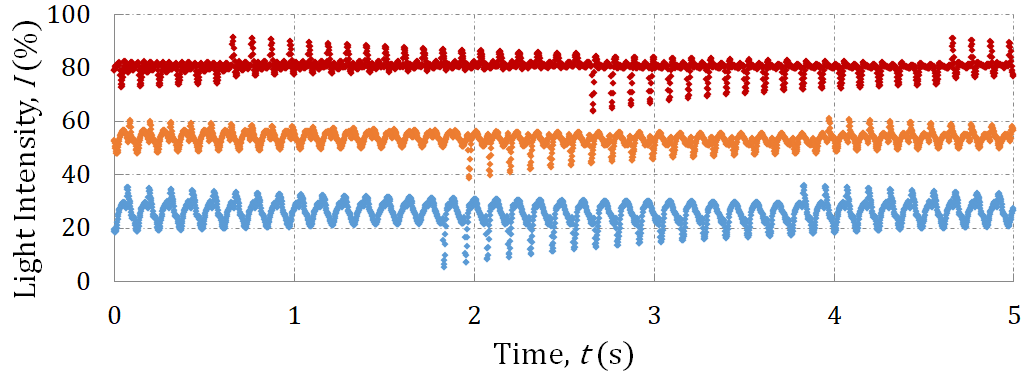
\includegraphics[width=2.8in]{LightIntensity.png}
    \caption{\textit{Solving for $v$ for various masses.} The blue points represent the amplitude vs time graph of the string with tension of (3.92 $\pm$ 0.01) N, the orange points represent a string with tension of (4.41 $\pm$ 0.01) N, and the red points represent a string with tension of (4.90 $\pm$ 0.01) N. Each curve is normalized about a different point so that they are easier to view.}
\end{figure}

\noindent We then find the time interval between each peak, $t$, and divide double the distance between the wave driver and pulley, $L$, by the time interval to solve for $v$:

\begin{table}[!htbp]
\caption{Experimental Wave Speeds}
\centering
\scalebox{0.7}{
\begin{tabular}{lllr}
\toprule
\multicolumn{2}{l}{$L$ = (3.060 $\pm$ 0.002) m} \\
\cmidrule{1-3}
Tension (N) & Time Interval (s) & Velocity (m/s) \\
\midrule
3.92 $\pm$ 0.01 & 0.122 $\pm$ 0.001 & 25.08 $\pm$ 0.04\\
4.41 $\pm$ 0.01 & 0.114 $\pm$ 0.001 & 26.84 $\pm$ 0.03\\
4.90 $\pm$ 0.01 & 0.106 $\pm$ 0.001 & 28.87 $\pm$ 0.03\\
\bottomrule
\end{tabular}}
\end{table}

\noindent The uncertainty of the experimental velocity is found using the following equation:

\footnotesize
\begin{equation}
\delta v = \sqrt{\bigg ( \frac{1}{t}\delta d \bigg )^2 + \bigg ( \frac{d}{t^2} \delta t \bigg)^2}
\end{equation}
\normalsize

\noindent The following table compares the predicted values of velocity with the experimental ones:

\begin{table}[!htbp]
\caption{Wave Speed Comparison}
\centering
\scalebox{0.7}{
\begin{tabular}{lllr}
\cmidrule{1-3}
Tension (N) & Predicted (m/s) & Experimental (m/s) \\
\midrule
3.92 $\pm$ 0.01 & 24.6 $\pm$ 1.1 & 25.08 $\pm$ 0.04\\
4.41 $\pm$ 0.01 & 26.3 $\pm$ 0.9 & 26.84 $\pm$ 0.03\\
4.90 $\pm$ 0.01 & 28.1 $\pm$ 1.0 & 28.87 $\pm$ 0.03\\
\bottomrule
\end{tabular}}
\end{table}

\noindent The next part of the lab involved attempting to find the fundamental mode of a standing wave with the two fixed ends of the string being the clamp and the pulley. We begin by testing driving frequencies around a predicted resonance frequency using the following equation:

\footnotesize
\begin{equation}
f = \frac{nv}{2L}
\end{equation}
\normalsize

\noindent Where $n$ refers to the harmonic number, $v$ is the velocity of a transverse wave on the string, and $L$ is the length of the string. Plugging in our experimental values into the above equation, we estimate the frequency for the fundamental mode of the string to be around 9.43 Hz.

\noindent We then try several frequencies in the ballpark of the estimated frequency to find the frequency of the fundamental mode. By observing which frequency produces the largest amplitude, we are then able to find the frequency associated with the fundamental mode. We find that a driving frequency of (9.540 $\pm$ 0.003) Hz produces the largest amplitude of standing waves.

\noindent Via the usage of Lissajous figures, we then verify the accuracy of the experimental resonance frequency. While the Lissajous figures are not in the form of ellipses, we are still able to ``measure" a form of symmetry by viewing how much the figure shifts over time. We define a symmetric figure as one that traces approximately the same path with each iteration.

\begin{figure}[!htbp]
    \centering
    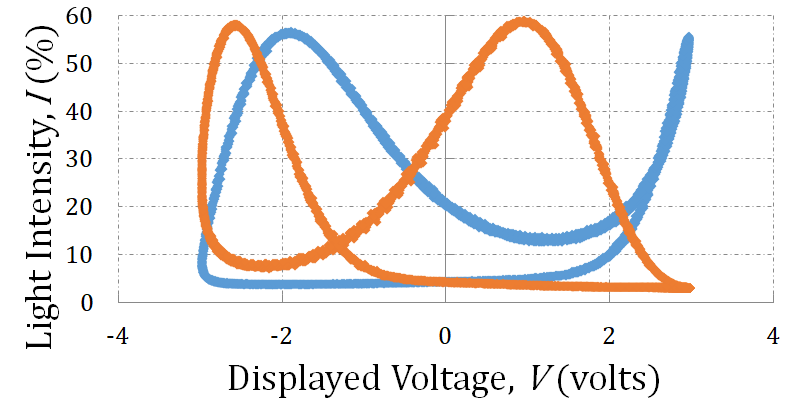
\includegraphics[width=2.8in]{Lissajous.png}
    \caption{\textit{Verification of harmonic frequencies.} The orange points and blue points represent Lissajous figures corresponding to driving frequencies of 19.08 Hz and 28.62 Hz, respectively. These represent the $n=2$ and $n=3$ modes, respectively.}
\end{figure}

\noindent We use this method of verification as we find the harmonics for increasing $n$ values (refer back to Equation 8). Furthermore, we note that $n-1$ nodes appear between the two end nodes of the string as we increase harmonics.

\noindent Using the above verification methods, we find the $n = 2, 3, 4,$ and $5$ frequencies to be equal to 19.08 Hz, 28.62 Hz, 38.16 Hz, and 47.70 Hz, respectively. We note that as the harmonic modes increase, the amplitude of oscillation decreases.

\noindent Next, we pinch the string at the midpoint, therefore artificially creating a node at the point. We find that for the even values of $n$, there is little effect to the amplitude of oscillation of the string, as there is already naturally a node at that point. However, for odd $n$ values such as $n=5$, we find that the amplitude of oscillation almost disappears entirely. This is due to the fact that by preventing oscillation at that point, we are effectively enforcing a new boundary condition onto the string. Therefore, the conditions that were used to calculate the fundamental mode no longer apply.

\noindent We also note that we were only able to visually identify nodes and anti-nodes to approximately the 9th mode. At that point, the amplitude of oscillation becomes negligible to the point at which visually there are no longer any nodes or antinodes.

\noindent Finally, we attempt to create a node at the point where the photodiode is located over the string. The laser is approximately 50 mm from the pulley, and therefore, the end of the string. We also know that each mode creates $2^{n-1}$ equally spaced nodes between the two nodes that make up the end of the string. From this, we can use math to predict which mode would create a node any point.

\noindent If we take the total length of the string, 1580 mm, and divide it by 50 mm to partition it into $m$ equally spaced 50 mm portions, we find that we divide it into ~32 portions. 32 is equal to $2^5$, and using that knowledge, we can therefore predict that the 6th mode will create a node 50 mm from the end of the string. When we input a driving frequency of 57.24 Hz, we see that a node is indeed created at that point.

%------------------------------------------------

\section{Discussion}

\noindent When we compare the experimental and the predicted values of the transverse waves on the string, we see that there is a notable difference between the values. However, they nonetheless fall within the uncertainties of each other, and despite the large uncertainties, none of them exceed 5\% of the value.

\hfill

\noindent When we view the experiment as a whole, we can note that there are many sources of systematic uncertainty within it. The effects of a possible source of systematic uncertainty can be seen within the calculations for the fundamental frequency: regardless of whether the experimental or predicted transverse velocity was used in Equation 6, we find that the calculated fundamental frequency of the string to be lower than the experimental one. This can be associated with the photodiode and laser system.

\hfill

\noindent A second source of systematic uncertainty can be found during the section during which we clamp down the center of the string. As the clamp we use does not clamp a single point at the node, but rather instead has a definite width, it affects the amplitude of the even numbered harmonics as well - albeit not to the same extent as it does odd numbered harmonics.

\hfill

\noindent Finally, a third problem that became more prevalent as the driving frequency of the string increased was the horizontal motion of the string: as the string oscillated vertically, it also experienced horizontal motion that increased with driving frequency. This in turn affects the accuracy of the photodiode measurements, as the change in light intensity cannot be attributed to vertical motion alone.

%----------------------------------------------------------------------------------------
%	REFERENCE LIST
%----------------------------------------------------------------------------------------

\begin{thebibliography}{99} % Bibliography - this is intentionally simple in this template

\bibitem{1}
Campbell, W. C. \textit{et al}. Physics 4AL: Mechanics Lab Manual (ver. August 31, 2017).
(Univ. California Los Angeles, Los Angeles, California).

\end{thebibliography}

%----------------------------------------------------------------------------------------

\end{document}
